\section{Artificial Evolution and Development}
TODO rewrite

\textit{Artificial development} and \textit{artificial evolution} takes inspiration from biology in order to explore large and complex solution spaces for some given problem.

In a typical \textit{genetic algorithm} (GA) setup \cite{mitchell-2001},
relatively simple representations of solutions are encoded as \textit{genotypes} (also called \textit{genomes}).
Through some \textit{development process} a genotype may be transformed into a \textit{phenotype} which can be used to attempt to solve the problem at hand.
The performance of the phenotype at solving the problem is the \textit{fitness} of that individual genotype.

The fitnesses of a \textit{population} of different individuals are compared.
A selection process picks individuals from the population that get to reproduce.
This selection process is usually stochastic, with a bias towards picking the individuals with the highest fitness, but some chance of picking a less fit individual now and then.

Individuals that are selected for reproduction are paired up.
The genotypes of the pair are combined in some fashion to create a new genotype.
In addition to the combination, random mutations may also be applied in order to produce new features not present in either parent.
As new individuals are born, the older parent generation dies out, so that the entire population is replaced.
In some cases the very best individuals of the parent generation are cloned directly into the next generation,
ensuring that their well-performing genotype continues to be present until some better genotype comes along.
This is called \textit{elitism} \cite{vasconcelos2001improvements}.

Starting out with an arbitrary initial population and repeating this generational algorithm,
it is often possible to find novel genotypes that encode good solution to the problem at hand.
Like other algorithms that search a space of solutions,
there is a risk of getting stuck in a local maximum and never finding a global maximum,
an optimal solution to the problem at hand.
There are many kinds of parameters, such as mutation rate or selection function that can be tweaked to try to avoid this.

When a phenotype is developed into a genotype, it is either possible that the genotype encodes the entire phenotype explicitly,
or it is possible that the development process augments the information stored in the genotype to create a more complex phenotype.
This is called respectively \textit{direct} and \textit{indirect encoding} \cite{clune2011performance}.
Indirect encodings allows the evolutionary search to explore a space of genotypes that is smaller than the space of possible phenotypes.
This is the way development happens in nature, where simple genomes are developed into complex lifeforms \cite{clune2011performance}.

\subsection{NEAT}
\textit{NeuroEvolution of Augmenting Topologies} (NEAT) is a genetic algorithm variant introduced by Stanley and Miikkulainen in 2002 \cite{stanley-2002},
designed specifically to evolve ANNs.
When introducing CPPNs \cite{stanley-2007}, Stanley also introduced the CPPN-NEAT variation of the algorithm.

A NEAT genome consists of genes that encode nodes and connections between them.
Figure \ref{fig:neat} shows an example genotype to phenotype mapping.
NEAT starts with an initial population of very simple networks, typically with just the input and output nodes and connections between them.
Over generations, more nodes and vertices are added or disabled, activation functions are changed, and weights are adjusted.
The process of gradually expanding the genome is called \textit{complexification},
and reflects how life on earth is believed to have started with simple organisms and gradually evolved into more complex creatures \cite{darnell1986speculations,pross2005emergence}.

The genes that make up a NEAT genome are marked with an \textit{innovation number} so that they may be recognized as the same gene in different individuals.
As new features are added to the genomes, the individuals making up the population become gradually less similar.
The degree of similarity is measured through a measure called the \textit{compatibility distance}.
When the distance between individuals pass a certain threshold, they are segregated into separate species.
This process is called \textit{speciation}.
Pair selection for reproduction happens within species.
Typically the species that have the most fit individuals will produce more children,
while the less fit species will produce fewer (but not 0) children.

When a new species appears with a new feature,
the feature will not be tuned and likely affect the fitness of the individuals negatively.
NEAT protects new species for a certain amount of time,
allowing them time to adjust before being evaluated and, if performing poorly, being extincted to make more room for the more fit species.

\begin{figure}
\centering
\begin{subfigure}[t]{.5\columnwidth}
\centering
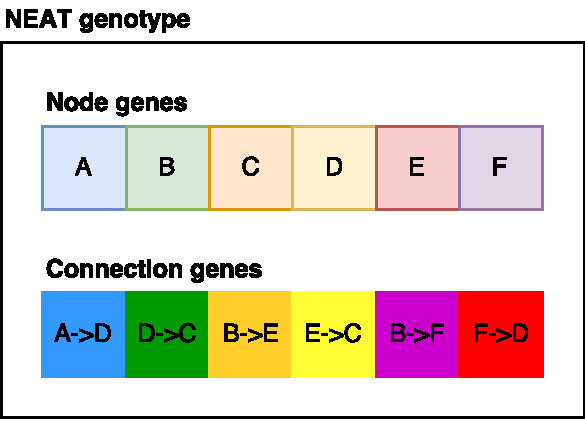
\includegraphics[height=5cm, keepaspectratio]{fig/NEAT_gt}
\caption{Genotype}
\end{subfigure}\hfill%
\begin{subfigure}[t]{.5\columnwidth}
\centering
\includegraphics[height=5cm, keepaspectratio]{fig/NEAT_pt}
\caption{Phenotype}
\end{subfigure}

\caption[Example NEAT genotype and phenotype]{
An example NEAT genotype and corresponding phenotype.
This example only shows the topology that the genotype encodes, leaving out the weights and activation functions.
}
\label{fig:neat}
\end{figure}

\begin{figure}
\centering
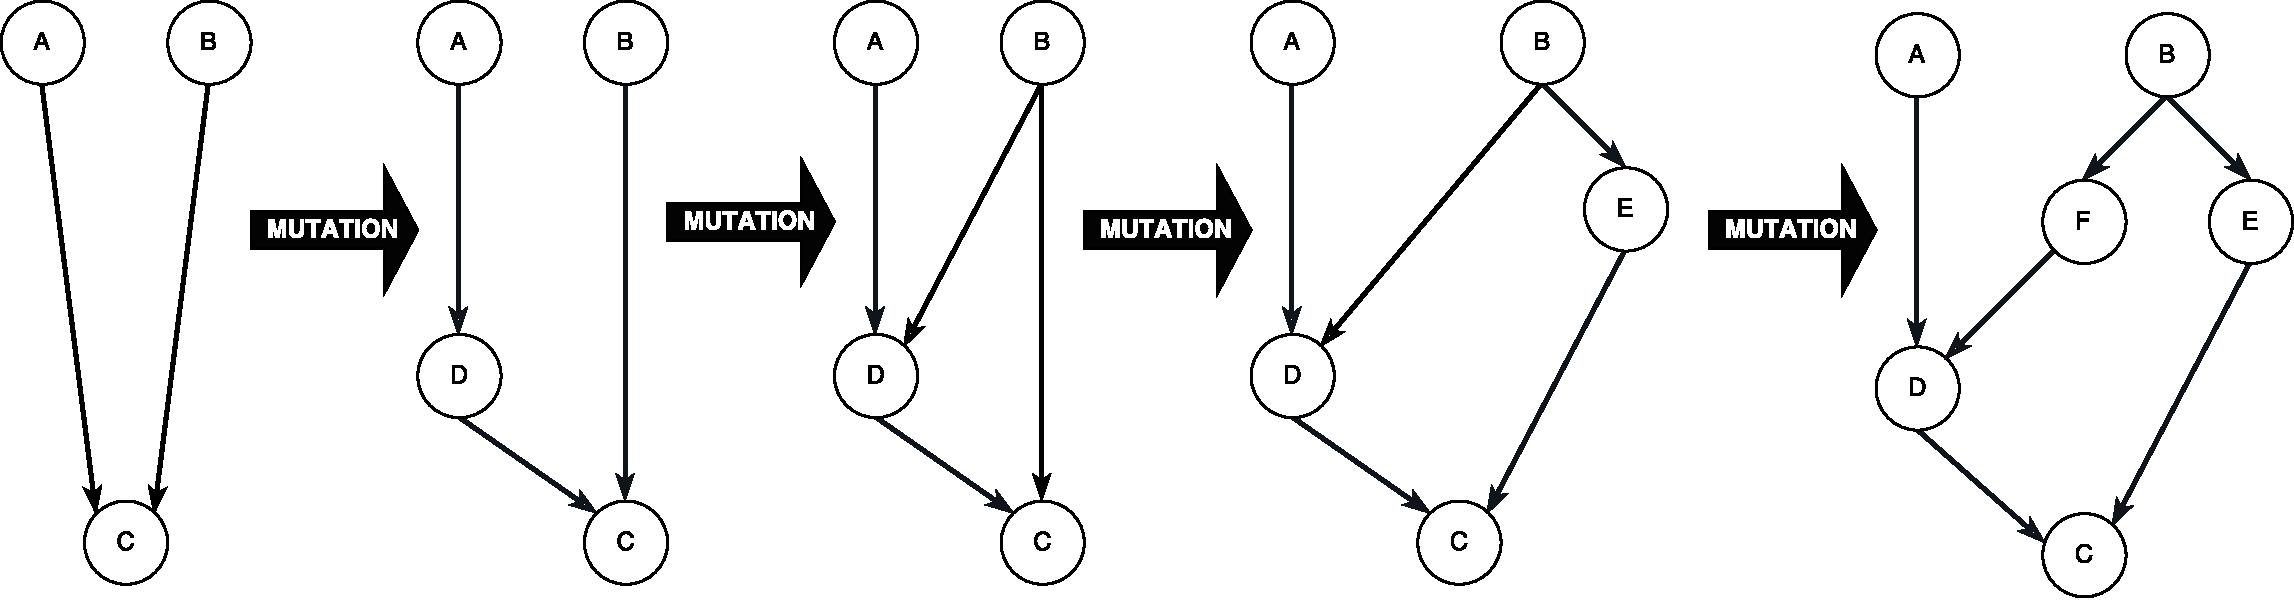
\includegraphics[width=\columnwidth, keepaspectratio]{fig/NEAT_mutation}
\caption[Example of NEAT mutation]{
    An illustrated example of NEAT mutation starting with a basic network of only two inputs and one output.
    Through the sequence neurons and connections are added until the network is equal to that in Figure \ref{fig:neat}.
    This example shows only mutation of genomes, leaving out the crossover operation which is also part of NEAT.
    }
\label{fig:neat_mutation}
\end{figure}


One notable use case of NEAT is called \textit{HyperNEAT} \cite{stanley2009hypercube}.
In this process, NEAT is used to evolve CPPNs whose output determine the topology of ANNs.
This is useful because it allows the ANN to scale easily, since the CPPN can just take more input and output more topology.
If the evolved CPPN has useful output at a small scale, it should also have a useful output at a large scale.

\subsection{Novelty Search}
\textit{Novelty search} is another genetic algorithm variant, introduced by Joel Lehmann and Kenneth O. Stanley in 2008 \cite{lehman-2008}.
It is good at \textit{deceptive} tasks, where local maximas in the fitness landscape do not lead to the global maximum, and thus "deceives" conventional algorithms.
Novelty search avoids this by eschewing the fitness measure entirely, and instead rewards \textit{innovation}, giving higher scores to genotypes that exhibit previously unseen behavior.
To find what behavior is new, an archive of seen behaviors is kept.
A \textit{distance metric} must be selected that is appropriate for the problem at hand.
For example, if the behavior of the phenotypes produces strings, an \textit{edit distance} measure such as the \textit{Levenshtein distance} can be used.
For each genotype the k nearest neighbors are found, and the average of these distances can be used as the \textit{novelty metric}.
If a new behavior is sufficiently novel, it is added to the archive.

TODO a bit more?
